\documentclass[10pt]{beamer}

\usepackage[utf8x]{inputenc}
\usepackage[T1]{fontenc}
\usepackage{lmodern}
\usepackage{microtype}
\usepackage{xspace}
%\usepackage[binary-units=true]{siunitx}
\usepackage{graphicx}
\usepackage{hyperref}
\usepackage{todonotes}
\usepackage{epstopdf}
\usepackage{array}
\usepackage{multicol}
\usepackage{multirow}
\usepackage{tabularx} 	% tabular with automatic line-break
\newcolumntype{Y}{>{\centering\arraybackslash}X} % centered column
\usepackage{amsmath}
\usepackage{grffile} 	% better name handling with graphicx
\usepackage{currfile} 	% provides relative file inclusion for tikzscale

\usepackage[]{algorithm2e}

\usepackage{tikz}
\usepackage{pgfplots}
\usepackage{tikzscale}
\pgfplotsset{compat=newest}
\usetikzlibrary{plotmarks}
\usepackage[absolute,overlay]{textpos}

% Math symbols
\usepackage{amsmath}
\usepackage{amssymb}
\usepackage{amsthm}
\DeclareMathOperator*{\argmin}{arg\,min}
\DeclareMathOperator*{\argmax}{arg\,max}
\newcommand\norm[1]{\left\lVert#1\right\rVert}

% Sets
\newcommand{\Z}{\mathbb{Z}}
\newcommand{\R}{\mathbb{R}}
\newcommand{\Rn}{\R^n}
\newcommand{\Rnn}{\R^{n \times n}}
\newcommand{\C}{\mathbb{C}}
\newcommand{\K}{\mathbb{K}}
\newcommand{\Kn}{\K^n}
\newcommand{\Knn}{\K^{n \times n}}

\newcommand\eqdef{\triangleq}

% Vectors
\newcommand{\vct}[1]{\boldsymbol{#1}}
\newcommand{\va}{\vct{a}}
\newcommand{\vb}{\vct{b}}
\newcommand{\vc}{\vct{c}}
\newcommand{\vd}{\vct{d}}
\newcommand{\ve}{\vct{e}}
\newcommand{\vf}{\vct{f}}
\newcommand{\vg}{\vct{g}}
\newcommand{\vh}{\vct{h}}
\newcommand{\vi}{\vct{i}}
\newcommand{\vj}{\vct{j}}
\newcommand{\vk}{\vct{k}}
\newcommand{\vl}{\vct{l}}
\newcommand{\vm}{\vct{m}}
\newcommand{\vn}{\vct{n}}
\newcommand{\vo}{\vct{o}}
\newcommand{\vp}{\vct{p}}
\newcommand{\vq}{\vct{q}}
\newcommand{\vr}{\vct{r}}
\newcommand{\vs}{\vct{s}}
\newcommand{\vt}{\vct{t}}
\newcommand{\vu}{\vct{u}}
\newcommand{\vv}{\vct{v}}
\newcommand{\vw}{\vct{w}}
\newcommand{\vx}{\vct{x}}
\newcommand{\vy}{\vct{y}}
\newcommand{\vz}{\vct{z}}
% Greek letter vectors
\newcommand{\valpha}{\vct{\alpha}}
\newcommand{\vbeta}{\vct{\beta}}
\newcommand{\vepsilon}{\vct{\epsilon}}
\newcommand{\vgamma}{\vct{\gamma}}
\newcommand{\vlambda}{\vct{\lambda}}
\newcommand{\vnu}{\vct{\nu}}
\newcommand{\vphi}{\vct{\phi}}
\newcommand{\vpsi}{\vct{\psi}}
\newcommand{\vtheta}{\vct{\theta}}
\newcommand{\vxi}{\vct{\xi}}
\newcommand{\vzero}{\vct{0}}
\newcommand{\vone}{\vct{1}}
% Matrices
\newcommand{\mtx}[1]{\boldsymbol{#1}}
\newcommand{\mzero}{\mtx{0}}
\newcommand{\mA}{\mtx{A}}
\newcommand{\mB}{\mtx{B}}
\newcommand{\mC}{\mtx{C}}
\newcommand{\mD}{\mtx{D}}
\newcommand{\mE}{\mtx{E}}
\newcommand{\mF}{\mtx{F}}
\newcommand{\mG}{\mtx{G}}
\newcommand{\mH}{\mtx{H}}
\newcommand{\mI}{\mtx{I}}
\newcommand{\mJ}{\mtx{J}}
\newcommand{\mK}{\mtx{K}}
\newcommand{\mL}{\mtx{L}}
\newcommand{\mM}{\mtx{M}}
\newcommand{\mN}{\mtx{N}}
\newcommand{\mO}{\mtx{O}}
\newcommand{\mP}{\mtx{P}}
\newcommand{\mQ}{\mtx{Q}}
\newcommand{\mR}{\mtx{R}}
\newcommand{\mS}{\mtx{S}}
\newcommand{\mT}{\mtx{T}}
\newcommand{\mU}{\mtx{U}}
\newcommand{\mV}{\mtx{V}}
\newcommand{\mW}{\mtx{W}}
\newcommand{\mX}{\mtx{X}}
\newcommand{\mY}{\mtx{Y}}
\newcommand{\mZ}{\mtx{Z}}

\usepackage{comment}
\usepackage{pgfpages}
\usepackage{bm}

\usetheme[progressbar=frametitle]{metropolis}
\tikzset{font={\fontsize{10pt}{12}\selectfont}}
\usepackage{hf-tikz}
\usetikzlibrary{ 
	calc,
	arrows,
	arrows.meta,
	automata, 
	shapes, 
	snakes, 
	positioning, 
	decorations,
	decorations.text,
	fit,
	matrix,
	mindmap
	}
\tikzstyle{noeud-std}=[draw,fill=black,circle,inner sep=0pt,minimum size=7pt]
\usepackage{tkz-graph}
\usepackage{xspace}
\usepackage{amsmath}
\usepackage{mathtools}

\definecolor{green}{HTML}{14B03D}
\newcommand{\payoff}[2]{{\color{green}#1}, {\color{red}#2}}

\usepackage{comment}
\usepackage{pgfpages}
\usepackage{bm}

\usetheme[progressbar=frametitle]{metropolis}
\tikzset{font={\fontsize{10pt}{12}\selectfont}}

\usepackage{xspace}
\usepackage{bm}
\usepackage{amsmath}
\usepackage{mathtools}

\newcommand{\gf}{\mathbb{F}_2}
\newcommand{\hw}[1]{\norm{#1}_\mathcal{H}}
\renewcommand{\ker}[1]{\text{Ker}\left(#1\right)}
\newcommand{\im}[1]{\text{Im}\left(#1\right)}

\title{LINMA2380 - Matrix computations}
\subtitle{A (really) quick introduction to coding theory}
\date{\today}
\author{Gaëtan Cassiers\and Antoine Paris}
\institute{Ecole polytechnique de Louvain}
\titlegraphic{\hfill
\includegraphics[height=1cm]{logo}}

\begin{document}
\maketitle

\section{Introduction and motivation}
\begin{frame}{What is coding theory?}
    \begin{itemize}
        \item Originally an \textbf{engineering problem}:
        \begin{center}
            ``\textit{Codes were invented to correct errors on noisy communication channels}''
            \cite{macwilliams}
        \end{center}
        \item Coding theory started in 1947 with the work of \textsc{Hamming},
        \textsc{Shannon} and \textsc{Golay}.
    \end{itemize}

    \begin{figure}[ht]
        \centering
        \begin{minipage}{0.32\textwidth}
            \centering
            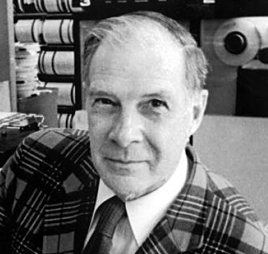
\includegraphics[width=0.79\textwidth]{img/hamming.jpg}
        \end{minipage}\hfill
        \begin{minipage}{0.32\textwidth}
            \centering
            
\includegraphics[width=\textwidth]{img/shannon.jpg}
        \end{minipage}\hfill
        \begin{minipage}{0.32\textwidth}
            \centering
            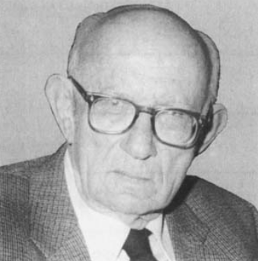
\includegraphics[width=0.74\textwidth]{img/golay.png}
        \end{minipage}
    \end{figure}
\end{frame}

\begin{frame}{How do we model this noisy communication channel?}
    \begin{block}{Binary symmetric channel (BSC)}
        \begin{figure}[h]
            \centering
            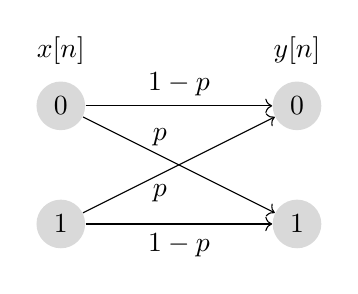
\begin{tikzpicture}
                \node at (0, 2.2) {$x[n]$};
                \node at (3, 2.2) {$y[n]$};
                \node (a) [circle, fill=gray!30] at (0,0) {1};
                \node (b) [circle, fill=gray!30] at (0,1.5) {0};
                \node (c) [circle, fill=gray!30] at (3,0) {1};
                \node (d) [circle, fill=gray!30] at (3,1.5) {0};
                \draw[->] (a) -- (c) node[pos=.5,sloped,below] {$1-p$};
                \draw[->] (a) -- (d) node[pos=.4,below] {$p$};
                \draw[->] (b) -- (c) node[pos=.4,above] {$p$};
                \draw[->] (b) -- (d) node[pos=.5,sloped,above] {$1-p$};
            \end{tikzpicture}
        \end{figure}
        \begin{itemize}
            \item $x[n]$ and $y[n]$ are the input and output \textbf{bit streams}
            \item the channel randomly flips bit with probability $p$, called the \textbf{bit
            error rate} (BER)
            \[ Pr\left[x[n] \neq y[n]\right] = p. \]
        \end{itemize}
    \end{block}
\end{frame}

\begin{frame}{Typical BER for uncoded communications}
    \begin{exampleblock}{Typical BER (uncoded communications)}
    For common communication channels (4G, WiFi, satellite...), typically
    \[ p = 10^{-1} \text{ to } 10^{-4} \]
    which (for 4G) would give at least \textbf{$10^4$ errors per second}:
    {\color{red}unacceptable}.
    \end{exampleblock}

    \begin{block}{Remark}
        $x[n], y[n] \in \gf$:
        \begin{itemize}
            \item $\gf$ is a field $(\{0, 1\}, +, \cdot)$
            \item $x + y = x \oplus y = x \text{ XOR } y = x + y \mod 2$
            \item $x \cdot y = x \text{ AND } y$
            \item $-x = x$, hence "-" is equivalent to "+"
        \end{itemize}
    \end{block}
\end{frame}

\section{A very basic example: repetition code}
\begin{frame}{A very basic example: repetition code (1)}
    Let's again consider a \textit{binary symmetric channel} (BSC) that flips a bit with a
    given probability $p$
    \begin{center}
        011... $\xrightarrow{\text{noisy channel}}$ 0{\color{red}0}1...
    \end{center}
    How can we detect and/or correct this error? \\
    $\to$ \textbf{We need to add some redundancy!}

    \begin{exampleblock}{Repetition code of order 3}
        Instead of transmitting a 0 (resp. a 1), transmit 000 (resp. 111). This defines a
        set of \textit{codewords} $\mathcal{C} = \{000, 111\}$.

        \begin{center}
            \begin{tabular}{c|c}
                \textbf{bit} & \textbf{codeword} \\
                \hline
                0   & 000 \\
                1   & 111
            \end{tabular}
        \end{center}
    \end{exampleblock}
\end{frame}

\begin{frame}{A very basic example: repetition code (2)}
    \begin{exampleblock}{Back to our example}
        If a single error occurs, we can correct it by majority voting in each block
        of 3 successive bits
        \begin{center}
            011... $\xrightarrow{\text{coding}}$ 000|111|111...
            $\xrightarrow{\text{noisy channel}}$
            {\color{red}1}00|1{\color{red}0}1|11{\color{red}0}...
        \end{center}
        The \textbf{error-correcting capability} is equal to 1.
    \end{exampleblock}
\end{frame}


\section{Let's formalize a bit all this...}
\begin{frame}{Definitions and notations}
    \begin{block}{Notations}
        \begin{itemize}
            \item $\vu = (u_1\cdots u_k)$ denotes a $k$-length \textit{message} we want to transmit
            \item $\vx = (x_1\cdots x_n)$ denotes an $n$-length \textit{codeword} that we send over
            the noisy channel
            \item $\mathcal{C} \subset \gf^n$ is the set of all possible codewords.
        \end{itemize}
    \end{block}
    
    \begin{block}{Definitions}
        \begin{itemize}
            \item The \textbf{length} of a code is $n$.
            \item The \textbf{rank} of a code is $k$.
            \item The \textbf{rate} of a code, noted $R$, is defined as
            \[ R \eqdef k/n. \]
        \end{itemize}
    \end{block}

    \begin{exampleblock}{Example}
        For a repetition code of order 3: $k = 1$, $n = 3$, $R = 1/3$.
    \end{exampleblock}
\end{frame}

\begin{frame}{Hamming distance and minimal distance}
    \begin{block}{Definitions}
        \begin{itemize}
            \item The \textbf{Hamming weight} of a vector $\vx = (x_1\cdots x_n)$ is the number
            of non-zero $x_i$ and is denoted by $\hw{\vx}$.
            \item The \textbf{Hamming distance} between two vectors $\vx = (x_1\cdots x_n)$ and
            $\vy = (y_1\cdots y_n)$ is the number of places where they differ and is
            $\hw{\vx-\vy}$.
            \item The \textbf{minimal distance} of a code is the minimum Hamming distance between
            its codewords and is denoted $d$
            \[ d = \min_{\vx\neq \vx' \in \mathcal{C}} \hw{\vx-\vx'}. \]
        \end{itemize}
    \end{block}

    \begin{exampleblock}{Example}
        For a repetition code of order 3, $\mathcal{C} = \{000, 111\} \Rightarrow d = 3$.
    \end{exampleblock}
\end{frame}

\begin{frame}{Error correcting capability}
    \begin{block}{Theorem}
        A code with minimum distance $d$ can correct $\lfloor\frac{1}{2}(d-1)\rfloor$ errors.
    \end{block}

    \begin{exampleblock}{Example}
        For a repetition code of order 3,
        \begin{center}
            000, 001, 010, 100 $\xrightarrow{\text{decoding}}$ 0, 0, 0 \\
            111, 110, 101, 011 $\xrightarrow{\text{decoding}}$ 1, 1, 1. 
        \end{center}
        This code can thus correct 1 error.
    \end{exampleblock}
\end{frame}

%\begin{frame}{A more involved example}
%    Let the set of codewords $\mathcal{C}$ be given by
%    \[ \mathcal{C} = \{000000, 111000, 001110, 100011, 010101\} \]
%    \begin{exampleblock}{It's quizz time}
%        \begin{itemize}
%            \item What is the code length $n$? \pause \textbf{6} \pause
%            \item What is the minimal distance of the code $d$? \pause \textbf{3} \pause
%            \item What is the error-correcting capability? \pause \textbf{1}
%        \end{itemize}
%    \end{exampleblock}
%\end{frame}

\section{Great. Now, how is this related to matrices?}
\begin{frame}{Linear codes}
    \begin{block}{What is a linear code?}
        Let's consider a code $\mathcal{C}$ of length $n$ and rank $k$.
        The code $\mathcal{C}$ is said to a $\textit{linear code}$ if it is a
        $k$-dimensional vector subspace of $\gf^n$.
    \end{block}

    \begin{exampleblock}{You already know a linear code! Any guess?}
        \pause
        Our good old repetition code of order 3 is a linear code. Indeed,
        $\mathcal{C} = \{000, 111\}$ is a $1$-dimensional vector subspace of
        $\gf^3$.
    \end{exampleblock}
\end{frame}

\begin{frame}{Properties of linear codes: generator matrix}
    \begin{block}{Generator matrix}
        Let $\mathcal{C}$ be a linear code with basis $(\vg_1, ..., \vg_k)$. The
        \textit{generator matrix} $\mG \in \gf^{n\times k}$ is given by
        \[ \mG = [\vg_1, \cdots, \vg_k] \]
        and the set of codewords $\mathcal{C}$ is the image of $\mG$
        \[\mathcal{C} = \im{\mG}. \]
        For each input message $\vu$, the corresponding codeword is given by
        \[ \vx = \mG\vu. \]
    \end{block}

    \begin{exampleblock}{Example}
        For a repetition code of order 3, $\mG = \begin{bmatrix} 1 & 1 & 1\end{bmatrix}^T$.
    \end{exampleblock}
\end{frame}

\begin{frame}{Properties of linear codes: parity check matrix}
    \begin{block}{Parity check matrix}
        There exists a matrix $\mH \in \gf^{(n-k)\times n}$, called the \textit{parity
        check matrix}, such that
        \[ \mathcal{C} = \ker{\mH}. \]
        This gives a set of equations that each codeword $\vx \in \mathcal{C}$ must satisfy
        \[ \mH\vx = 0. \]
    \end{block}
    
    \begin{exampleblock}{Example}
        For a repetition code of order 3,
        \[ \mH =
        \begin{bmatrix}
            1 & 1 & 0 \\
            1 & 0 & 1
        \end{bmatrix}. \]
        The parity check equations are $x_1 = x_2$ and $x_2 = x_3$ which indeed implies
        $x_1 = x_2 = x_3$.
    \end{exampleblock}

    \textbf{NB} $G$ and $H$ are not uniquely defined.
\end{frame}

\begin{frame}{We know how to encode. Now, how can we decode?}
    \begin{center}
        $\vu \xrightarrow{\text{encoder}} \vx \xrightarrow{\text{channel}} \vy \xrightarrow{\text{decoder}} \vy' \xrightarrow{} \vu'$
    \end{center}
    At the output of the binary symmetric channel, we get $\vy \in \gf^n$, a corrupted
    version of $\vx$
    \[ \vy = \vx + \ve \]
    where $\ve$ is the \textit{error vector}: \[\text{Pr}[e_i = 1] = p.\]

    The decoder decides from $\vy$ which codeword $\vx$ was sent.

    \begin{exampleblock}{Maximum likelihood decoding}
        Obviously, the decoder can't be certain of what $\ve$ was. It will thus
        choose the \textbf{most likely}. And it can be shown the most likely $\ve$
        is the one with minimal Hamming weight.
    \end{exampleblock}
\end{frame}

\begin{frame}{Decoding: more mathematically}
    Maximum likelihood decoding looks for the \textbf{closest codeword} $\vy' \in
    \mathcal{C}$
    \[ \argmin_{\vy'\in\mathcal{C}} \hw{\vy'-\vy}, \]
    or
    \[\argmin_{\mH\vy' = 0} \hw{\vy'-\vy}. \]
    
    \begin{alertblock}{Complexity}
        \begin{itemize}
            \item Brute-force requires to go through the $2^k$ possible codewords $\vu' \in
            \mathcal{C}$ and select the closest one for each received codewords.
            \item Tabulating results for all $\vy'$ is not possible neither, this would
            require a table of size $2^n$.
        \end{itemize}
        {\color{red}$\rightarrow$ not acceptable in both case}.
    \end{alertblock}    
\end{frame}

\begin{frame}{Syndrome decoding to the rescue}
    Remember that $\vy = \vx + \ve$ with $\ve$ the \textit{error vector}.
    \begin{block}{Definition}
        The \textbf{syndrome} of $\vy$ is defined as
        \[ \vs \eqdef \mH\vy = \mH\ve. \] 
    \end{block}
    Maximum likelihood decoding then reduces to
    \[ \argmin_{\mH\ve = \vs}\hw{\ve}. \]
    \begin{exampleblock}{Complexity}
        Given $\vy$, we can compute the syndrome $\vs$ efficiently. Since $\vs \in \im{\mH}$,
        there are $2^{n-k}$ possible syndromes: results can now be tabulated.
    \end{exampleblock}
    \begin{block}{Example}
        For Hamming code of redundancy $r$: $n = 2^r-1$, $k = 2^r-r-1$, $n-k = r$.
    \end{block}
\end{frame}

\section{A quick view on more complex stuff}

\begin{frame}{Well-known code families}
    \begin{itemize}
        \item There exists a lot of code families (not all codes
        are linear!): Hamming, Golay, Hadamard, BCH, Reed-Solomon
        (defined on $\mathbb{F}_{2^q}$), Justensen, etc.
        \item Construction of new codes from existing ones: dual codes, puncturing,
        expurgating, augmenting, etc.
    \end{itemize}    
\end{frame}

\begin{frame}{Longer codes}
    \begin{center}
        ``\textit{One version of the main problem of coding theory is to find codes
        with large rate (for efficiency) and large minimal distance (to correct
        many errors). Of course these are conflicting goals.}''
        \cite{macwilliams}
    \end{center}

    For practical purposes, we also want codes that can be efficiently encoded and decoded.

    \begin{exampleblock}{Low Density Parity Codes (LDPC)}
        Invented by \textsc{Gallager} at MIT in 1960, LDPC offers efficient iterative decoding
        thanks to a \textbf{sparse parity matrix} $\mH$
        (many "0", $\norm{\mH}_F \in \mathcal{O}(n)$).
        The code length of LDPC varies from $10^3$ up to $10^7$.
    \end{exampleblock}
\end{frame}

\begin{frame}{How important is this? (1)}
    \begin{exampleblock}{Example}
        In communication systems, the goal is to achieve the \textbf{minimal bit error rate}
        (BER) \textbf{for a given signal-to-noise ratio} (SNR). Coding offers what we call the...
        \textbf{coding gain}.
        \begin{figure}[ht]
            \centering
            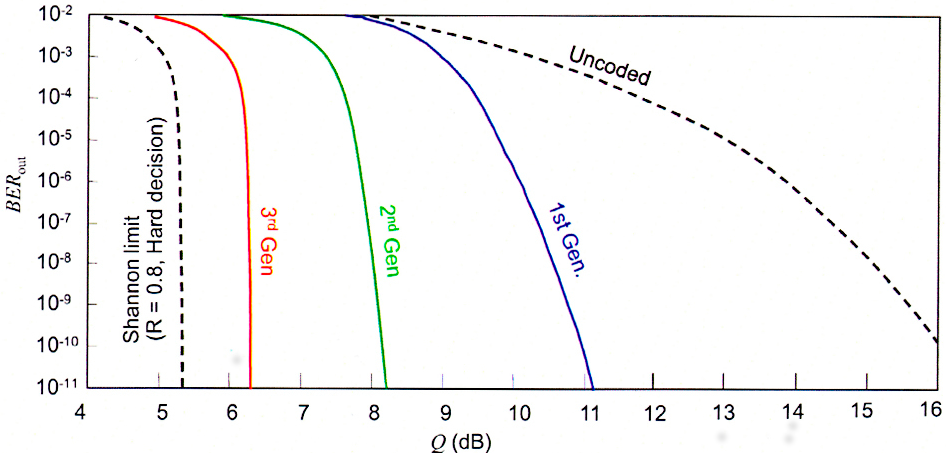
\includegraphics[width=0.8\textwidth]{img/example-com.png}
        \end{figure}
    \end{exampleblock}
\end{frame}

\begin{frame}{How important is this? (2)}
    Today, error-correcting codes are present in:
    \begin{itemize}
        \item \textbf{communications}: WiFi, 4G, Satellite, DSL...
        \item \textbf{storage devices}: HDD, SSD, CD/DVD/blu-ray...
        \item RAM, computer busses, GPUs...
    \end{itemize}
    and even applications in cryptography and quantum computing.
\end{frame}

\begin{frame}{References}
    \nocite{*}
    \bibliography{biblio}
    \bibliographystyle{plain}
\end{frame}

\begin{frame}[standout]
    Questions?
\end{frame}

\end{document}
